\section{Rupture: An improved attack}\label{subsec:rupture}
Our contributions include the development of a production-grade framework for
implementing this class of attacks called Rupture. Rupture was developed as
part of the work on extending the BREACH attack against modern systems and block
ciphers.

Rupture provides extended functionality regarding the network aspects of the
attack. It offers the ability to inject malicious code in any computer in the
network, as well as traffic inspection and analysis of captured packet lengths.

In addition, Rupture enables the automated computation of the reflection strings
in each stage of the attack.  It also amplifies the attack by issuing multiple
requests per candidate symbol in the alphabet $\Sigma$ in order to demonstrate
better probability of success. This is achieved by grouping requests in
samplesets, where each sampleset contains requests on a symbol in the alphabet
$\Sigma$. Requests in a sampleset may be constructed to enable optimization
methods described in \ref{subsec:blockalign} and \ref{subsec:parallel}.

The encrypted data pertaining to one response is a \textit{sample}. The set of
samples collected for a particular work are a \textit{sampleset}. A work
represents the set of requests needed per candidate in the secret's alphabet.

The attack is conducted in \textit{rounds}. In each round, a decision is made
about the state of the attack and more becomes known about the secret. In a
round, either the next byte of the secret becomes known, or the known alphabet
is drilled down to a smaller set. In order to compare various different
candidate alphabets, the attack executes a series of \textit{batches} of data
collection for each round.

In each batch, several works are issued and samples are collected from each
probability distribution pertaining to a candidate alphabet, forming a
sampleset. When samplesets of the same amount of samples have been collected for
all the candidate alphabets, a batch is complete and the data is analyzed. The
analysis compares the samples of different candidates and decides which is
optimal, i.e. which candidate is contains the correct guess. This decision is
made with some \textit{confidence} which is expressed in bytes. If the
confidence is insufficient, an additional batch of samplesets is collected, and
the analysis is redone until the confidence is sufficient.

Once enough batches have been collected for a decision to be made with good
confidence, the round of the attack is complete, since new information about the
secret have become known.

\subsection{Architecture}\label{app:rupture}
Rupture is a service-based architecture framework which contains multiple
independent components. While the components are designed to be able to run
independently on different networks or computer systems, easy instances of the
attack can be performed by running all subsystems on an individual system.

The framework assumes a \textit{target} service to be attacked. Typically
this target is a web service which uses TLS and
provides HTTPS endpoints. However, this assumption can
be relaxed and attacks against other similar protocols are possible. Any
protocol that exchanges encrypted data on the network and for which
the attack assumptions hold can in principle be attacked using Rupture. We
designed Rupture to be a good playground for experimentation for such new
attacks. Examples of other encrypted protocols for experimentation
include SMTP and XMPP.

The attack also assumes a user of the target service for which data will be
decrypted, the \textit{victim}. The victim is associated with a particular
target.

There are two underlying assumptions in our attack: The injection and the
sniffing assumptions. These are often, but not necessarily, achieved through the same means.

The injection assumption states that the adversary is able to inject code to the
victim's machine for execution. This code is able to issue adaptive requests to
the target service. Injection in Rupture is implemented by the
\textit{injector} component. The code that is injected is the \textit{client}
component.

The sniffing assumption states that the adversary is able to observe encrypted network
traffic between the victim and the target.
Sniffing is achieved through the \textit{sniffer}component.

The client must issue adaptive requests. For this purpose, it receives commands
through a \textit{command-and-control} channel. These commands are sent to the
client from the \textit{realtime} component with which the client maintains a
persistent connection.

The realtime component is only responsible for communicating with the client.
The actual decisions for the attack are driven by the \textit{backend}, which
maintains a persistent attack state. The backend stores persistent data in a
\textit{database} and receives data from the sniffer to perform analyses.

The various components are described in detail in the next sections.

\subsubsection{Client}

The client component is a Javascript code that issues requests towards a chosen
endpoint. This endpoint serves as the reflection oracle of the attack. The client
needs to be executed from the browser of the victim that the adversary is trying
to steal secrets from. That way, the victim's authentication cookies are
included in the request and the secrets are included in the
response.

The client contains minimal logic. It connects to the realtime service through
a command-and-control channel and registers itself. Then it waits
for work instructions by the command-and-control channel. The
client does not take any decisions or receive data about the progress of the
attack other than the work it is requested to do.
This allows the system to be upgraded without having to deploy a
new client at the victim's network.

As a regular user is browsing the Internet, multiple clients will be
injected in insecure pages and run under various contexts. All of
them register and maintain an open connection through a
with the realtime service. The realtime
service will activate one of them for this victim while keeping the others
dormant. The activated one will then receive work instructions. If the enabled
client dies, for example by closing the browser
tab, one of the rest of the clients will be woken up to continue the
attack.

\subsubsection{Injector}

The injector component is responsible for injecting the client to the victim's
browser. The injection is performed by ARP spoofing the local
network and forwarding all traffic in a Man-in-the-Middle manner. The fact that all HTTP
responses are infected increases robustness.

The injector component runs on the victim network and is
light-weight and stateless. It can be easily deployed on a small machine and
used for massive attacks. Multiple injectors can be deployed to different
networks, all controlled by the same central command-and-control channel.

\subsubsection{Realtime}

The realtime service is a service which awaits for work requests by clients. It
can handle multiple targets and victims. It receives command-and-control
connections from various clients which may live on different networks,
orchestrates them, and tells them which ones will remain dormant and which ones
will receive work, enabling one client per victim.

It maintains open web socket connections with clients and
connects to the backend service, facilitating the communication between the two
ends.

\subsubsection{Sniffer}

The sniffer component is responsible for collecting data from the
victim's network. As the client issues the requests, the sniffer
collects the ciphertext of the requests and responses as they
travel on the network. This encrypted data is then transmitted to the backend
for further analysis and decryption.

The sniffer exposes an HTTP API which is utilized by the backend for controlling
when sniffing starts, when it is completed, and retrieving the sniffed data.

\subsubsection{Backend}

The backend component is a Python code that controls the attack execution. It
initializes the attack and calculates the request sets that should be
collected. It is responsible for strategic decision taking, statistical
analysis of collected samples, adaptively advancing the attack, and storing
persistent data about the attacks in progress for future analysis.

It communicates with the realtime component in order to guide the client as to
what requests need to be made at each stage of the attack. Meanwhile, it orders
the sniffer to listen and report network traffic, which stored
at the end of each phase of the attack. The backend analyzes the
network data and calculates the confidence in the success for the attack. At the
end of each round, the predicate $Q$ is detected, depending on which method of
the ones described
in \ref{subsec:reflectionmethods} is used.

   \begin{figure}[thpb]
      \centering
          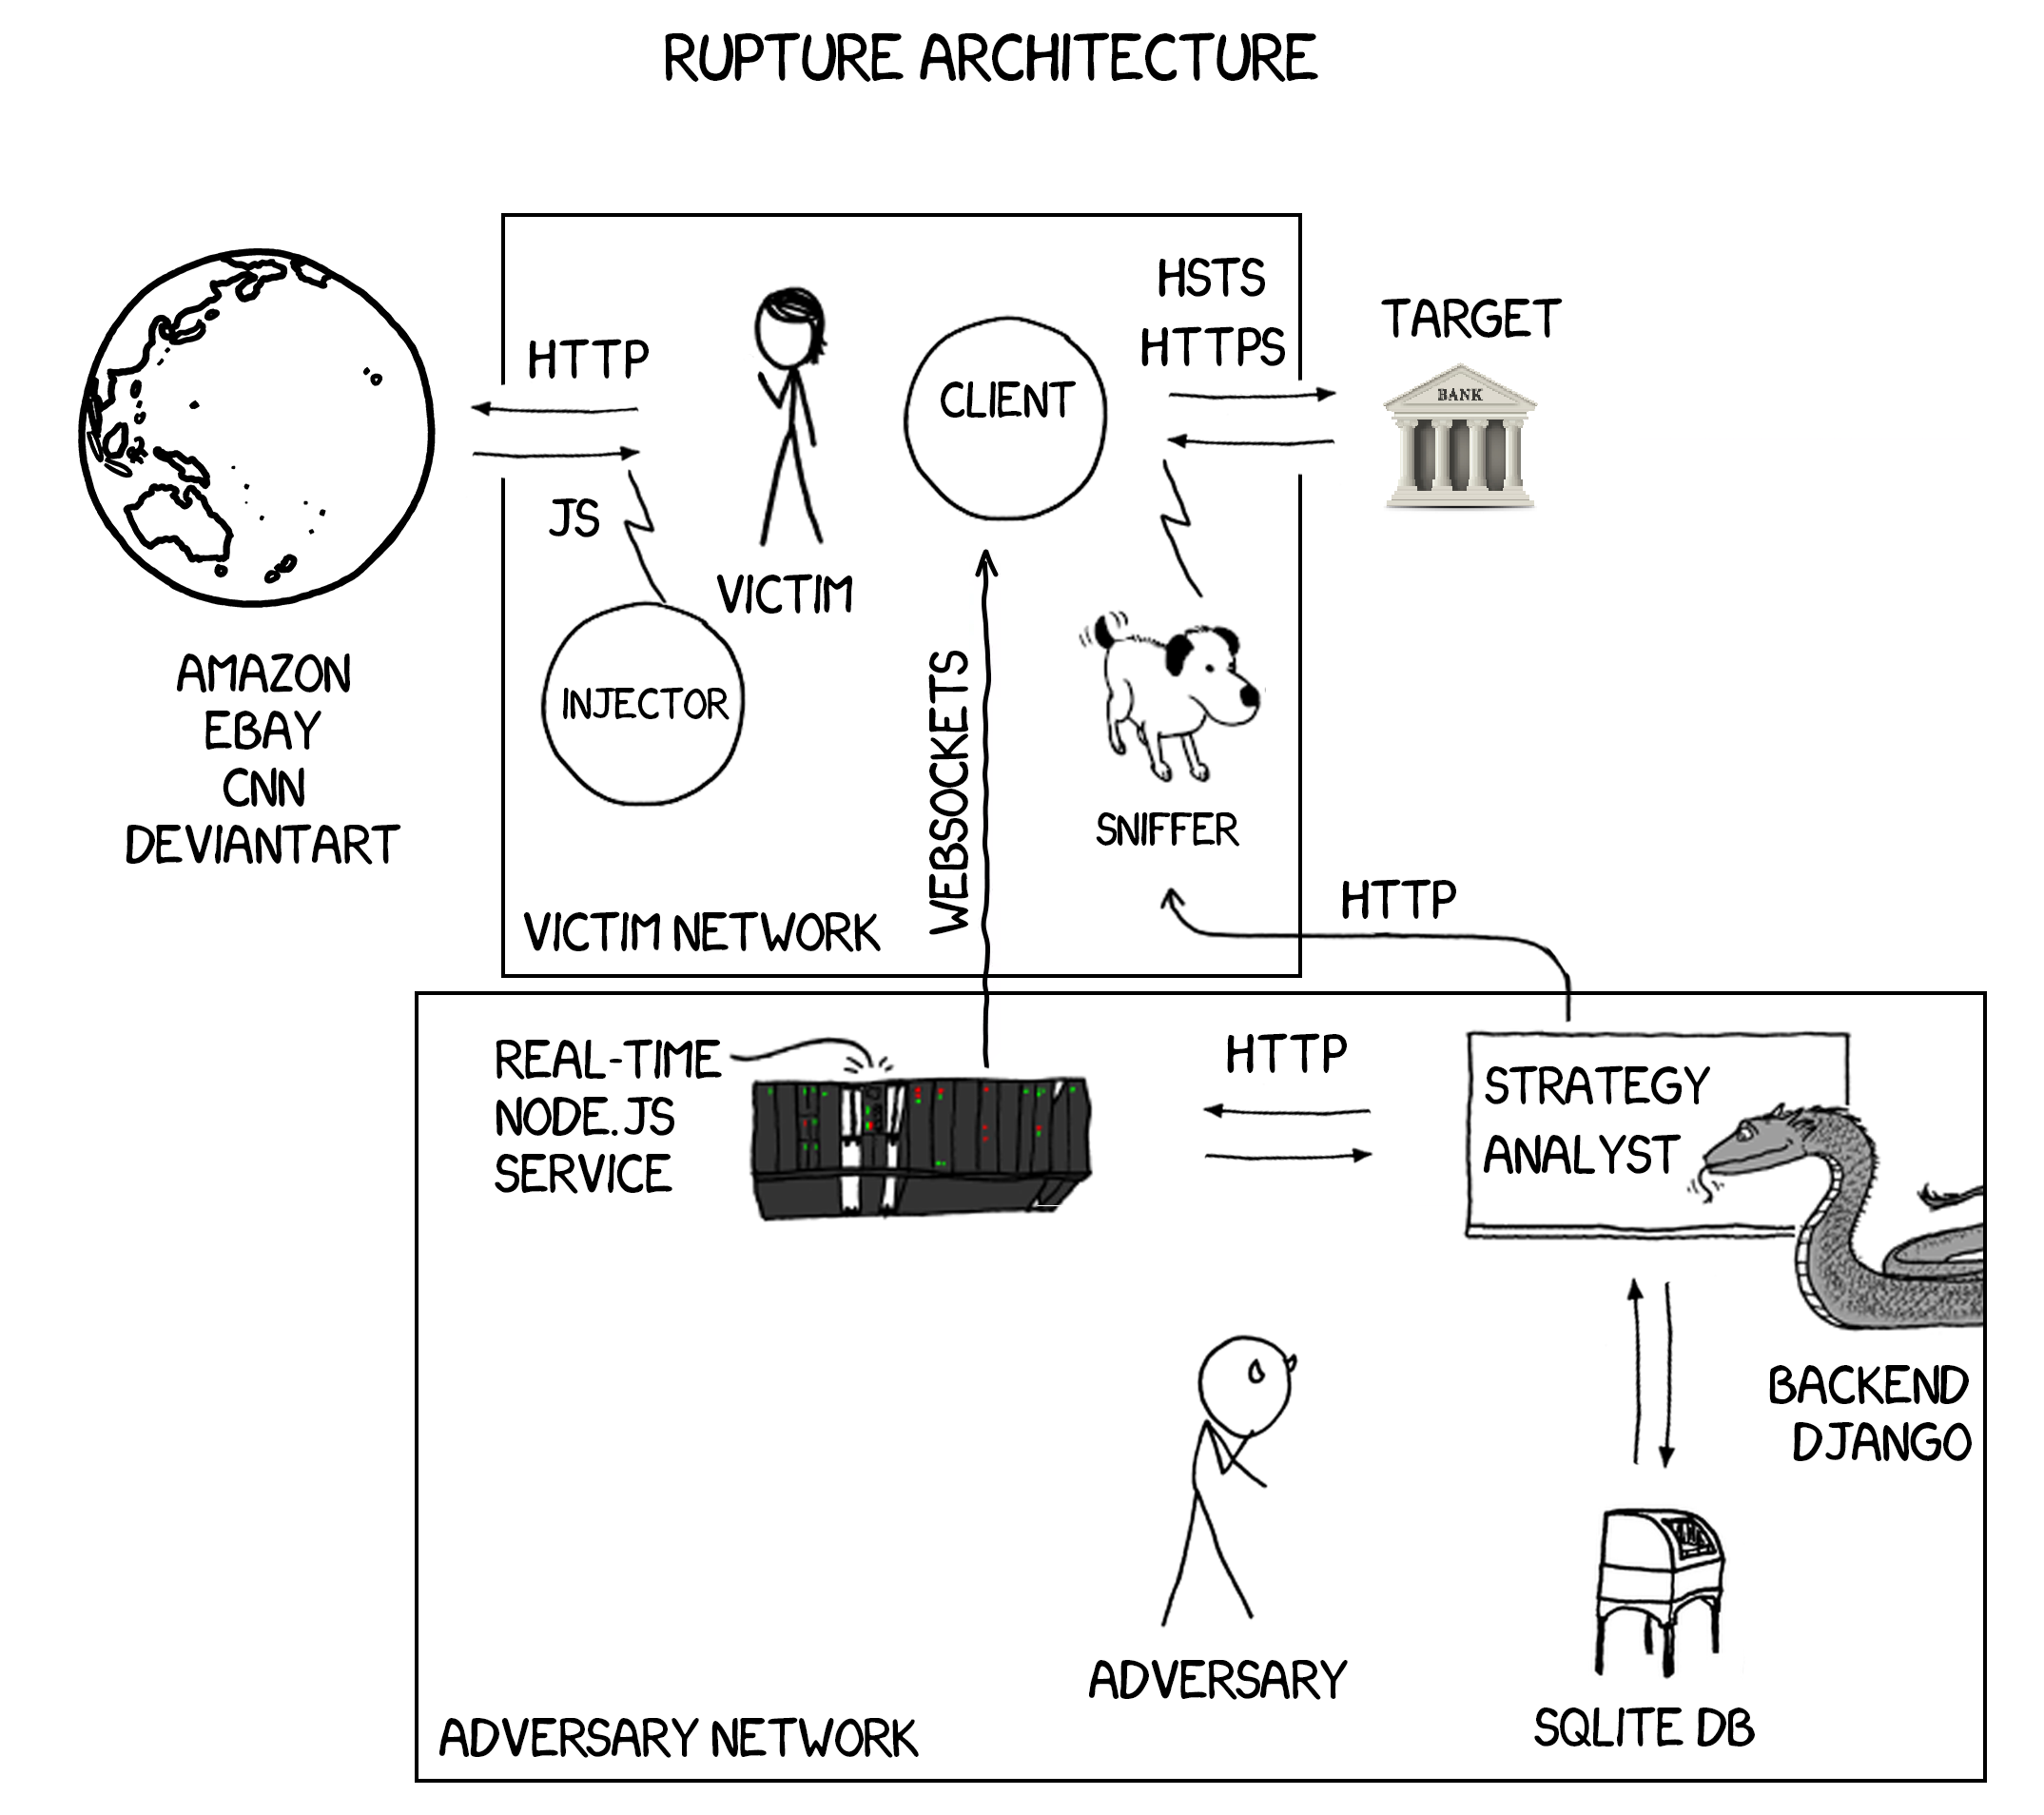
\includegraphics[width=0.48\textwidth]{figures/architecture.png}
      \caption{Rupture Architecture}
   \end{figure}
